\subsection{Верхня оцiнка загального вiдновлюючого спектрального числа для графа кактуса}

Для довільного зваженого графа кактуса ${\bf G}$, зображеного на рисунку \ref{Cactus:image}, і $G\neq C_n$ розглянемо поставлену задачу.
\begin{figure}[H]
    \centering
    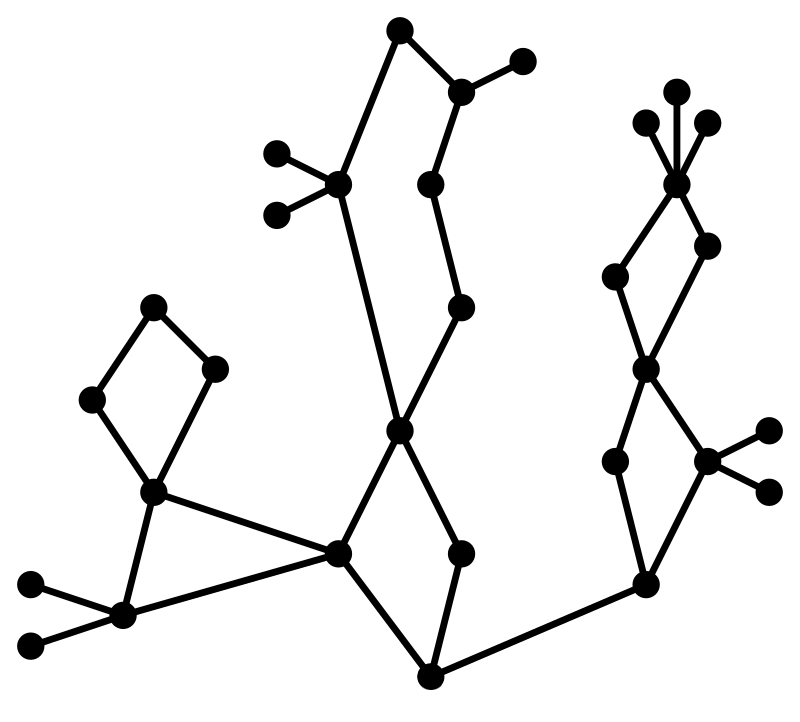
\includegraphics[width=0.45\linewidth]{pictures/Cactus.png}
    \caption{\textbf{G} --- граф кактус}
    \label{Cactus:image}
\end{figure}
Нехай $c$ --- це кількість циклів у графі кактусі. Видалимо $c$ ребер, тобто одне ребро з кожного циклу, що інцидентній вершині, у якої степінь більше або дорівнює трьом. Отримаємо дерево $H$ і застосуємо теорему 4. Тобто за $cv(H)$ підспектрами, де $cv$ --- кількість висячих вершин, можна відновити ваги на дереві $H$. І $cv(H)$ дорівнює $cv(G)+c$, оскільки з видаленням ребра з одного циклу кількість висячих вершин збільшується на 1, а ми видаляємо ребро $c$ разів. Ще треба $c$ підспектрів, щоб відновити $c$ ребер, які ми видалили.

Отже, $srn(G) \leq cv(G) +2c$.